\documentclass[letterpaper]{article} % DO NOT CHANGE THIS
\usepackage[submission]{aaai2027}  % DO NOT CHANGE THIS
% The serif, sans-serif, and monospaced fonts are loaded automatically by
% aaai2027.sty (newtxtext, helvet, courier). DO NOT add \usepackage{times},
% \usepackage{helvet}, \usepackage{courier}, or any other font package.
\usepackage[hyphens]{url}  % DO NOT CHANGE THIS
\usepackage{graphicx} % DO NOT CHANGE THIS
\urlstyle{rm} % DO NOT CHANGE THIS
\def\UrlFont{\rm}  % DO NOT CHANGE THIS
\usepackage{natbib}  % DO NOT CHANGE THIS AND DO NOT ADD ANY OPTIONS TO IT
\usepackage{caption} % DO NOT CHANGE THIS AND DO NOT ADD ANY OPTIONS TO IT
\usepackage{amsmath,amssymb}
\frenchspacing  % DO NOT CHANGE THIS


%
% These are recommended to typeset algorithms but not required. See the subsubsection on algorithms. Remove them if you don't have algorithms in your paper.
\usepackage{algorithm}
\usepackage{algorithmic}

%
% Recommended for better-looking tables
\usepackage{booktabs}

%
% Keep the \pdfinfo as shown here. There's no need
% for you to add the /Title and /Author tags.
\pdfinfo{
/TemplateVersion (2027.1)
}

% DISALLOWED PACKAGES
% \usepackage{authblk} -- This package is specifically forbidden
% \usepackage{balance} -- This package is specifically forbidden
% \usepackage{CJK} -- This package is specifically forbidden
% \usepackage{float} -- This package is specifically forbidden
% \usepackage{flushend} -- This package is specifically forbidden
% \usepackage{fullpage} -- This package is specifically forbidden
% \usepackage{geometry} -- This package is specifically forbidden
% \usepackage{hyperref} -- This package is specifically forbidden
% \usepackage{navigator} -- This package is specifically forbidden
% (or any other package that embeds links such as navigator or hyperref)
% \usepackage{indentfirst} -- This package is specifically forbidden
% \usepackage{layout} -- This package is specifically forbidden
% \usepackage{multicol} -- This package is specifically forbidden
% \usepackage{nameref} -- This package is specifically forbidden
% \usepackage{savetrees} -- This package is specifically forbidden
% \usepackage{setspace} -- This package is specifically forbidden
% \usepackage{stfloats} -- This package is specifically forbidden
% \usepackage{tabu} -- This package is specifically forbidden
% \usepackage{titlesec} -- This package is specifically forbidden
% \usepackage{tocbibind} -- This package is specifically forbidden
% \usepackage{ulem} -- This package is specifically forbidden
% \usepackage{wrapfig} -- This package is specifically forbidden
% DISALLOWED COMMANDS
% \nocopyright -- Your paper will not be published if you use this command
% \addtolength -- This command may not be used
% \balance -- This command may not be used
% \baselinestretch -- Your paper will not be published if you use this command
% \clearpage -- No page breaks of any kind may be used for the final version of your paper
% \columnsep -- This command may not be used
% \newpage -- No page breaks of any kind may be used for the final version of your paper
% \pagebreak -- No page breaks of any kind may be used for the final version of your paper
% \pagestyle -- This command may not be used
% \tiny -- This is not an acceptable font size.
% \vspace{- -- No negative value may be used in proximity of a caption, figure, table, section, subsection, subsubsection, or reference
% \vskip{- -- No negative value may be used to alter spacing above or below a caption, figure, table, section, subsection, subsubsection, or reference

\setcounter{secnumdepth}{0} %May be changed to 1 or 2 if section numbers are desired.
\hbadness=10000
\vbadness=10000
\hfuzz=20pt

% The file aaai2027.sty is the style file for AAAI Press
% proceedings, working notes, and technical reports.
%

% Title

% Your title must be in mixed case, not sentence case.
% That means all verbs (including short verbs like be, is, using,and go),
% nouns, adverbs, adjectives should be capitalized, including both words in hyphenated terms, while
% articles, conjunctions, and prepositions are lower case unless they
% directly follow a colon or long dash
\title{CalveKV: Cross-Layer Adaptive Latent Vector Eviction for Efficient LLM Inference}
\author{
    %Authors
    % All authors must be in the same font size and format.
    Written by AAAI Press Staff\textsuperscript{\rm 1}\thanks{With help from the AAAI Publications Committee.}\\
    AAAI Style Contributions by Peter Patel Schneider,
    Sunil Issar,\\
    J. Scott Penberthy,
    George Ferguson,
    Hans Guesgen,
    Francisco Cruz\equalcontrib\corresponding,
    Marc Pujol-Gonzalez\equalcontrib\corresponding
}
\affiliations{
    %Afiliations
    \textsuperscript{\rm 1}Association for the Advancement of Artificial Intelligence\\
    % If you have multiple authors and multiple affiliations
    % use superscripts in text and roman font to identify them.
    % For example,

    % Sunil Issar\textsuperscript{\rm 2},
    % J. Scott Penberthy\textsuperscript{\rm 3},
    % George Ferguson\textsuperscript{\rm 4}\corresponding,
    % Hans Guesgen\textsuperscript{\rm 5}
    % Note that the comma should be placed after the superscript

    1101 Pennsylvania Ave, NW Suite 300\\
    Washington, DC 20004 USA\\
    % email address must be in roman text type, not monospace or sans serif
    proceedings-questions@aaai.org
%
% See more examples next
}

%Example, Single Author, ->> remove \iffalse,\fi and place them surrounding AAAI title to use it
\iffalse
\title{My Publication Title --- Single Author}
\author {
    Author Name
}
\affiliations{
    Affiliation\\
    Affiliation Line 2\\
    name@example.com
}
\fi

\iffalse
%Example, Multiple Authors, ->> remove \iffalse,\fi and place them surrounding AAAI title to use it
\title{My Publication Title --- Multiple Authors}
\author {
    % Authors
    First Author Name\textsuperscript{\rm 1,\rm 2}\equalcontrib,
    Second Author Name\textsuperscript{\rm 2}\equalcontrib,
    Third Author Name\textsuperscript{\rm 1}\corresponding
}
\affiliations {
    % Affiliations
    \textsuperscript{\rm 1}Affiliation 1\\
    \textsuperscript{\rm 2}Affiliation 2\\
    firstAuthor@affiliation1.com, secondAuthor@affilation2.com, thirdAuthor@affiliation1.com
}
\fi


\begin{document}

\maketitle

\begin{abstract}
Despite the exceptional capabilities of Large Language Models (LLMs) in handling long contexts, the memory overhead associated with Key-Value (KV) caching during autoregressive inference remains a primary bottleneck for high-throughput deployment. 

Recent architectural innovations—specifically the Multi-Head Latent Attention (MLA) mechanism introduced in DeepSeek-V2/V3—have significantly alleviated this issue by compressing KV states into low-rank latent vectors. However, generation tasks involving ultra-long contexts still demand further memory optimization. Existing token eviction strategies primarily target uncompressed, traditional KV caches; applying them directly to MLA would necessitate decompressing the latent space, thereby negating MLA's inherent memory efficiency advantages. To address this, we propose "CalveKV," a novel, highly generalizable, and scalable algorithm that operates efficiently directly within the compressed latent space. 

Our experiments reveal a phenomenon of "Cross-layer Persistence" regarding latent vector importance: the importance of latent vectors determined in shallower Transformer layers serves as a reliable prior for attention distributions in deeper layers. Specifically, by applying a composite scoring function based on the L2-norm and variance of latent features at a designated early decision layer (e.g., Layer 4), our algorithm enables the safe, global physical truncation of redundant latent vector caches across all subsequent layers. Extensive experiments on long-text and code corpora demonstrate the method's effectiveness. Latent Eviction introduces negligible computational overhead; it further compresses peak memory usage to 50–60 percent of the original MLA baseline while maintaining Time-to-First-Token (TTFT) and prefill latency. Crucially, this extreme compression does not compromise model accuracy, maintaining robust retrieval performance in "Needle In A Haystack" (NIAH) evaluations. Code and artifacts are withheld for double-blind review and will be released upon acceptance.
\end{abstract}

\section{Introduction}

Large Language Models (LLMs) have rapidly expanded the practical context length of neural text generation, enabling stronger performance on retrieval-heavy reasoning, long-form code completion, and document-grounded generation. Yet, for autoregressive decoding, the memory footprint of the Key-Value (KV) cache remains a central systems bottleneck. As sequence length grows, KV states scale linearly with the number of processed tokens and become the dominant memory consumer, directly constraining batch size, throughput, and deployability under fixed GPU budgets.

Architectures such as DeepSeek-V2/V3 partially mitigate this bottleneck through Multi-Head Latent Attention (MLA), which stores compressed latent representations instead of conventional full KV tensors. While MLA substantially improves memory efficiency, ultra-long context generation still faces strict memory limits in realistic serving scenarios. A natural direction is token eviction, but most existing eviction methods are designed for uncompressed KV caches. Applying those strategies to MLA generally requires decompression or proxy reconstruction, which undermines the primary efficiency advantage of latent-space caching.

This paper introduces \textbf{CalveKV}, a latent-native eviction framework that performs global cache reduction directly in the compressed space. The key observation is a cross-layer persistence effect: token importance estimated from latent statistics in shallower layers provides a reliable prior for deeper-layer attention allocation. Based on this observation, CalveKV computes a composite importance score from latent feature norm and variance at an early decision layer, then executes safe physical truncation of low-importance latent vectors for all subsequent layers. This design avoids repeated per-layer re-scoring and avoids decompressing latent caches.

CalveKV is designed for deployment efficiency rather than architectural redesign. It is model-compatible, lightweight, and easy to integrate into existing MLA inference pipelines. Empirically, on long-text and code-centric workloads, CalveKV reduces peak cache memory to approximately 50--60\% of the MLA baseline, while preserving Time-to-First-Token (TTFT), prefill latency, and downstream retrieval quality (including Needle-In-A-Haystack settings).

Our main contributions are as follows:
\begin{itemize}
  \item We identify and validate \emph{cross-layer persistence} of latent token importance in MLA-based Transformers, providing a practical signal for early-layer cache decisions.
  \item We propose \textbf{CalveKV}, a compressed-space eviction algorithm that combines latent norm and variance into a unified score and performs globally consistent truncation across later layers.
  \item We show that substantial memory compression can be achieved with negligible runtime overhead and without measurable degradation in long-context retrieval behavior.
\end{itemize}

These results suggest that latent-space eviction is a viable path toward scalable long-context LLM serving, complementing architectural compression with systems-level cache control.

% Uncomment the following to link to your code, datasets, an extended version or similar.
% You must keep this block between (not within) the abstract and the main body of the paper.
% Make sure that you do not de-anonymize yourself with these links.
% \begin{links}
%     \link{Code}{Anonymous repository (to be released upon acceptance)}
%     \link{Artifacts}{Anonymous supplementary materials (to be released upon acceptance)}
% \end{links}

% ─────────────────────────────────────────────────────────────────────────────
\section{Background and Related Work}

The attention mechanism utilized in Transformers continues to serve as the predominant cornerstone of contemporary large language models, with the corresponding KV cache compression emerging as a frequently debated topic in current research. The MLA algorithm represents a novel and highly efficient compression approach.

\subsection{Multi-Head Latent Attention}

DeepSeek-V2/V3 \cite{deepseekv2,deepseekv3} introduce \emph{Multi-Head Latent
Attention} (MLA) to alleviate the KV-cache bottleneck through a low-rank
bottleneck projection. Rather than caching full-rank key and value tensors, MLA
compresses each hidden state into a compact \emph{KV latent vector}:

\begin{equation}
  \mathbf{c}_{t}^{KV} = W^{DKV}\,\mathbf{h}_t,
    \quad \mathbf{c}_{t}^{KV} \in \mathbb{R}^{d_c},
  \label{eq:kv_compress}
\end{equation}

where $d_c \ll n_h d_h$ is the latent rank (e.g., $d_c\!=\!512$ for
DeepSeek-V2-Lite). During inference, content keys/values are reconstructed only
implicitly, while positional information is carried by a decoupled RoPE key.
Thus, the physical cache stores only
$(\mathbf{c}_{t}^{KV},\,\mathbf{k}_{t}^{R})$ per token—a total of
$d_c + d_R = 576$ scalars for DeepSeek-V2-Lite—compared with the
$2n_h d_h = 4096$ scalars required by standard MHA, achieving roughly a
$7\times$ memory reduction.

\paragraph{Weight Absorption at Inference.}
Materialising expanded keys/values for all cached tokens at every decoding step
would nullify this saving. MLA avoids this through \emph{weight absorption}: a
portion of the key up-projection is absorbed into the query projection,

\begin{equation}
  \tilde{\mathbf{q}}_{t,i}
    = {W^{UK}}^{\top}\mathbf{q}_{t,i}^{C}
    \in \mathbb{R}^{d_c},
  \label{eq:q_absorb}
\end{equation}

so content attention can be computed directly against cached latents:

\begin{equation}
  {\mathbf{q}_{t,i}^{C}}^{\!\top}\mathbf{k}_{j,i}^{C}
    = {\mathbf{q}_{t,i}^{C}}^{\!\top} W^{UK}\,\mathbf{c}_{j}^{KV}
    = \tilde{\mathbf{q}}_{t,i}^{\top}\,\mathbf{c}_{j}^{KV}.
  \label{eq:weight_absorb_k}
\end{equation}

The same idea applies on the value path: aggregation is first done in latent
space, then projected once. This \emph{zero-decompression inference} property is
fundamental to
CalveKV: importance scoring, eviction, and attention all operate directly on
$\mathbf{c}^{KV}$, without ever expanding the stored representations.

\subsection{KV Cache Compression}

Despite MLA's architectural efficiency, serving LLMs in ultra-long-context
regimes ($T \gg 32\text{k}$) still strains GPU memory. A complementary line of
work studies \emph{cache compression}, largely orthogonal to architectural
changes.

\subsubsection{Token Eviction.}
Token-eviction methods remove KV entries with low estimated future utility.
\citeauthor{zhang2023h2o}\shortcite{zhang2023h2o} show that a small set of
\emph{heavy hitters} captures most cumulative attention and maintain a fixed
budget of such tokens (H$_2$O). SnapKV \cite{li2024snapkv} uses a short
pre-generation observation window to select representative tokens, while
PyramidKV \cite{cai2024pyramidkv} allocates progressively smaller budgets in
deeper layers based on layer-wise sparsification. StreamingLLM
\cite{xiao2024streamingllm} further shows that a small set of \emph{attention
sink} tokens (often leading positions) should always be retained, which aligns
with CalveKV's sink-protection design.

Their shared limitation is reliance on \emph{expanded} key--value tensors. In
MLA, this would require decompressing $\mathbf{c}_{t}^{KV}$ into
$\mathbf{k}_{t}^{C}$ and $\mathbf{v}_{t}^{C}$ for scoring, partially restoring the
memory cost MLA is meant to avoid.

\subsubsection{Quantization.}
Quantization reduces per-entry storage through lower precision. KVQuant
\cite{hooper2024kvquant} reports sub-2-bit representations with non-uniform
per-channel quantization, and HqeKV \cite{yang2024hqekv} jointly optimizes
precision and eviction under a unified importance objective. However, because
quantization preserves token count, it does not reduce the
$\mathcal{O}(T)$ decoding bandwidth cost.

\subsection{Residual-Compensated Eviction: IndexMem}

IndexMem \cite{indexmem2024} mitigates eviction-induced information loss by
compressing the representations of evicted tokens into a compact
\emph{latent memory module} that is injected as a residual bias into subsequent
attention outputs.  However, IndexMem operates on conventional expanded KV
tensors: applying it within an MLA system would require first decompressing
$\mathbf{c}_{t}^{KV}$ into full-rank $\mathbf{k}^C,\mathbf{v}^C$, partially
negating MLA's $7\times$ memory advantage and introducing additional
inference-time state.  CalveKV avoids this by performing all scoring and
truncation natively in the compressed latent space, with no auxiliary
data structures.

\paragraph{Summary.}
All existing cache compression methods were designed for uncompressed KV
tensors and require decompression overhead within an MLA system.  CalveKV
fills this gap by operating intrinsically in the latent space, enabling
zero-decompression eviction.
% ─────────────────────────────────────────────────────────────────────────────

\section{Method}

\subsection{Overview}

CalveKV is a latent-space cache eviction method designed for MLA inference. For a given prefill 
data block, the method stores each token as a compressed latent cache entry containing RoPE 
components, computes importance directly within the latent space, and executes a unified global 
eviction decision. 


\begin{figure*}[!t]
  \centering
  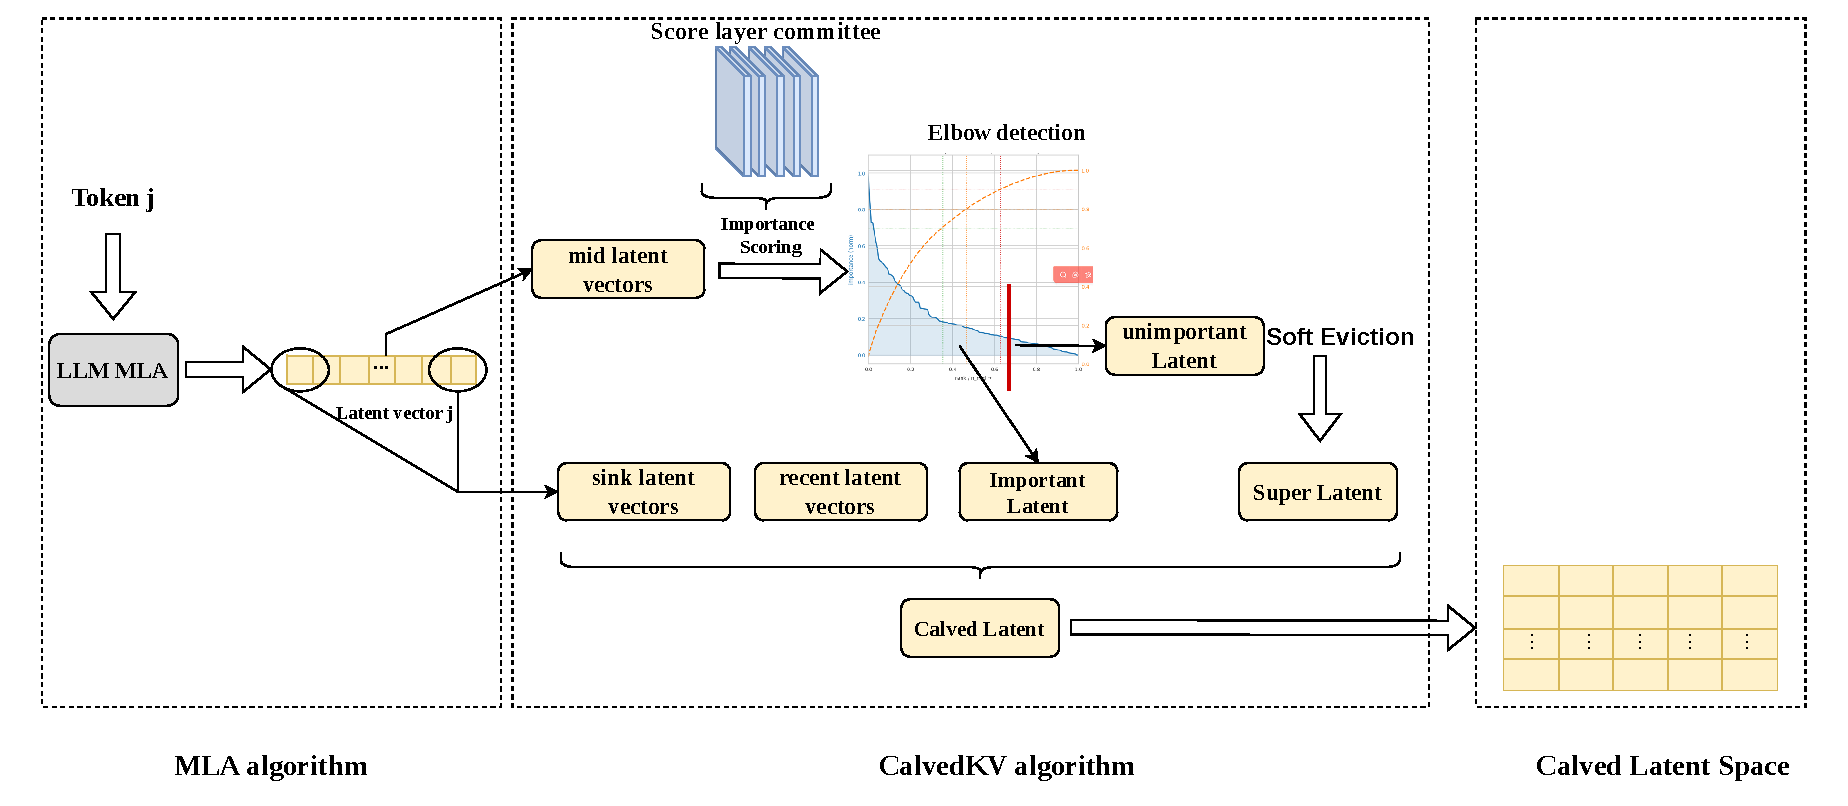
\includegraphics[width=\linewidth]{Figures/222.drawio.pdf}
  \caption{Overview of the CalveKV pipeline. The method performs latent-native scoring, cross-layer aggregation, and global cache eviction without reconstructing full K/V tensors.}
  \label{fig:overview}
\end{figure*}

The importance formula accounts for both the significance and the contribution 
of the latent vector to the output space. By default, the algorithm preserves "sink" latent vectors 
and recent latent vectors, while ranking intermediate latent vectors based on importance scores; 
experiments show that the importance distribution follows an "L-shaped" long-tail decay, prompting 
the use of a mechanism combining the "elbow method" and a safety net to determine which latent 
vectors to evict. Selected latent vectors may be merged into "super latent vectors" to preserve 
residual information. We observed that the importance distribution of LLM latent vectors exhibits 
cross-layer stability—with importance often determined at shallower layers—so we independently 
calculate importance scores across multiple shallow "score layers" (layers 4, 6, 8, 12, and 16), 
aggregate them via averaging at decision layer D=16, and share the resulting eviction decision 
across all layers. Finally, by concatenating the preserved and merged latent vectors from the 
beginning, end, and middle sections, we achieve significant compression of GPU memory usage.



The method contains two coupled components. Weight Absorption reuses the MLA
attention path without reconstructing full K/V tensors. On top of this latent
path, Query-Aware and Value-Aware scoring provides the ranking signal used by
the eviction policy.

\subsection{Query-Aware and Value-Aware Importance Scoring}

In Multi-head Latent Attention~\cite{deepseekv2}, the KV projection is
decomposed into a compression step and an up-projection step.
Given hidden state $\mathbf{h}_t$, a shared low-rank latent is computed as
$\mathbf{c}_t^{KV} = W_{DKV}\,\mathbf{h}_t \in \mathbb{R}^{R}$,
from which the content key and value are recovered:
\begin{equation}
  \mathbf{k}_t^C = W_{UK}\,\mathbf{c}_t^{KV},
  \qquad
  \mathbf{v}_t   = W_{UV}\,\mathbf{c}_t^{KV}.
\end{equation}
The content (RoPE-free) attention score between positions $i$ and $j$ is
\begin{equation}
  a_{ij}
  = \frac{(\mathbf{q}_i^C)^\top \mathbf{k}_j^C}{\sqrt{d}}
  = \frac{(\mathbf{q}_i^C)^\top W_{UK}\,\mathbf{c}_j^{KV}}{\sqrt{d}}.
  \label{eq:attn_std}
\end{equation}

\paragraph{Weight Absorption.}
By rearranging Eq.~\eqref{eq:attn_std} via the associative law, we define the
\emph{absorbed query}:
\begin{equation}
  \mathbf{q}_i^{\mathrm{abs}}
  \;\triangleq\; W_{UK}^\top\,\mathbf{q}_i^C
  \;\in\; \mathbb{R}^{H \times R},
  \label{eq:qabs}
\end{equation}
so that the attention score becomes
$a_{ij} = \bigl(\mathbf{q}_i^{\mathrm{abs}}\bigr)^\top \mathbf{c}_j^{KV}\!/\sqrt{d}$.
This reformulation allows importance scoring to operate directly on the cached
latent $\mathbf{c}_j^{KV} \in \mathbb{R}^{512}$ without ever materialising
the expanded key $\mathbf{k}_j^C \in \mathbb{R}^{H \times 128}$,
saving both memory and computation.

\paragraph{Causal Attention Column-Sum.}
Let $n$ denote the number of candidate tokens in the prefill
(excluding the protected sink and recency tokens).
We construct the causally masked logit matrix for head $h$:
\begin{equation}
  \hat{L}_{ij}^{(h)} =
  \begin{cases}
    \dfrac{\bigl(\mathbf{q}_i^{\mathrm{abs}}\bigr)^{(h)\top}
           \mathbf{c}_j^{KV}}{\sqrt{d}}
    & j \le i,\\[6pt]
    -\infty & j > i,
  \end{cases}
  \label{eq:logit}
\end{equation}
and compute row-wise attention probabilities
$P_{ij}^{(h)} = \operatorname{softmax}\!\bigl(\hat{L}_{i,\cdot}^{(h)}\bigr)_j$.
The importance score of token $j$ is its \emph{column sum} averaged over heads:
\begin{equation}
  s[j]
  = \frac{1}{H}\sum_{h=1}^{H}\sum_{i=j}^{n-1} P_{ij}^{(h)},
  \label{eq:colsum}
\end{equation}
which measures the cumulative causal attention token $j$ receives from all
subsequent positions.  A high $s[j]$ indicates that many future tokens rely
on $j$; a low value identifies it as a candidate for eviction.

\paragraph{Value-Aware Modulation.}
High-frequency function words can attract broad but shallow attention,
inflating $s[j]$ while contributing minimally to the model output.
We therefore modulate the column-sum score by the $\ell_2$ norm of the
token's value projection, which quantifies its magnitude of contribution
in the output space:
\begin{equation}
  \nu[j] = \bigl\|W_{UV}\,\mathbf{c}_j^{KV}\bigr\|_2,
  \qquad
  \bar\nu[j] = \frac{\nu[j]}{\frac{1}{n}\sum_{k}\nu[k] + \varepsilon}.
  \label{eq:valnorm}
\end{equation}
The final token importance score is
\begin{equation}
  \mathcal{I}[j]
  = \underbrace{s[j]}_{\text{how often attended}}
    \;\times\;
    \underbrace{\bar\nu[j]}_{\text{output contribution}}.
  \label{eq:importance}
\end{equation}
Tokens that attract sustained causal attention \emph{and} carry large value
projections are preserved; tokens with diffuse positional attention but
negligible value content are discounted.


%humanrized-----------------------------------------------------------------

\paragraph{Sink and Recency Token Protection.}
When processing latent vectors during the prefill phase, we choose to leave a portion of 
the vectors at the beginning and end unprocessed. And we will scoring and evicting only 
those latent vectors in the middle.

The protection at the beginning is \emph{Attention sinks} (first $N_s = 4$ tokens).
Empirical analysis reveals that the leading tokens in a sequence
accumulate disproportionately large cumulative attention weights
across all Transformer layers. This is a phenomenon widely attributed to the
``attention sink'' effect~\cite{xiao2024streamingllm}.
The most important reason is that these tokens do not exhibit correspondingly elevated
$\ell_2$ norms in the latent space, their $\|\mathbf{c}^{KV}\|_2$ values are
typically unremarkable, and their attention column sums under causal masking
are confined to positions $i > j$, which may be sparse for early tokens.
Consequently, any scoring criterion derived from latent statistics or our 
query-aware formulation of Eq.~\eqref{eq:importance} will
systematically under-value sink tokens, producing erroneous eviction.
These tokens are therefore excluded from the scoring pool and unconditionally
appended to the keep set.

The protection at the end is \emph{Recency tokens} (last $N_r = 16$ tokens).
Under causal attention, a token $j$ near the end of the prefill window
has been attended to by only a small number of subsequent positions, or none at all for the 
final token.
Its causal column sum
$s[j] = \frac{1}{H}\sum_{h}\sum_{i > j} P_{ij}^{(h)}$
is structurally small \emph{by construction}, the attention distribution over it
has not had sufficient opportunity to accumulate.
Query-aware scoring therefore systematically under-estimates the importance
of recent tokens, so these tokens are similarly excluded from scoring and unconditionally retained.

%-------------------------------------------------------------------------------------------------------

%hunamrized-------------------------------------------------------------------------------------------

Formally, we can denoting the protected sets as
\begin{equation}
  \mathcal{K}_{\mathrm{sink}}   = \{0,\,\ldots,\,N_s - 1\},
  \qquad
  \mathcal{K}_{\mathrm{recent}} = \{n - N_r,\,\ldots,\,n - 1\},
  \label{eq:protected}
\end{equation}
importance scoring and the subsequent adaptive budget determination are
applied only to the \emph{mid-token} interval
$\mathcal{M} = \{N_s,\,\ldots,\,n - N_r - 1\}$.
The final keep set is the union
\begin{equation}
  \mathcal{K}
  = \mathcal{K}_{\mathrm{sink}}
    \;\cup\;
    \mathcal{K}_{\mathrm{mid}}^{\star}
    \;\cup\;
    \mathcal{K}_{\mathrm{recent}},
  \label{eq:keepset}
\end{equation}
where $\mathcal{K}_{\mathrm{mid}}^{\star} \subseteq \mathcal{M}$ contains
the $k^{\star}$ mid-tokens selected by the scoring and adaptive budget
(Eq.~\eqref{eq:budget}).
This structure ensures that scoring noise at the sequence boundaries
never contaminates the eviction decision. The budget mechanism will focus
its adaptive logic exclusively on the informationally heterogeneous mid-range
tokens.

%----------------------------------------------------------------------------------------------

\paragraph{Query Subsampling for Long Sequences.}
The full $n \times n$ attention matrix in Eq.~\eqref{eq:logit} is
computationally infeasible at long context: with $n = 32\text{k}$,
$H = 16$ heads, and \texttt{float32} precision, it alone requires
${\sim}68\,\text{GB}$.
We uniformly sample $K \ll n$ query indices
from the $N$ available query rows, and use their column-sum statistics to
estimate the full attention column sum:
\begin{equation}
  I_j \approx \frac{N}{K}\cdot
  \frac{1}{H}\sum_{h=1}^{H}\sum_{k=1}^{K} P_{\mathrm{sample}(k),j}^{(h)}.
  \label{eq:sampled}
\end{equation}
By Monte Carlo estimation, the sample expectation is proportional to the full
expectation. Since eviction only requires relative ranking for Top-$k$
selection, the global scale factor $N/K$ does not affect ordering and can be
ignored in practice.
Consequently, computation and memory complexity are reduced from
$\mathcal{O}(Hn^2)$ to $\mathcal{O}(HKn)$;
with $K{=}512$, the $32\text{k}$-context case requires approximately $1\,\text{GB}$.






\subsection{Cross-Layer Shared Indices and Multi-Layer Committee Decision}

A fundamental systems constraint of MLA inference mandates that all Transformer
layers maintain \emph{identical} physical KV lengths: the underlying
\texttt{DynamicCache} concatenates cross-step entries layer-by-layer, and any
length mismatch raises a shape error at runtime. This forces a
\emph{globally shared} eviction decision: a single index set $\mathcal{K}$
must govern all layers simultaneously. Formally, let $\mathcal{I}^{(\ell)}[j]$
denote the importance score of token $j$ at layer $\ell$. A single-layer policy
selects one layer $\ell^{\star}$ and defines
\begin{equation}
  \mathcal{K}
  = \operatorname{TopB}\!\left(\mathcal{I}^{(\ell^{\star})}\right)
    \cup \mathcal{K}_{\mathrm{sink}} \cup \mathcal{K}_{\mathrm{recent}},
\end{equation}
where $\operatorname{TopB}(\cdot)$ retains the top-$B$ scored mid-range tokens,
and sink/recency tokens are unconditionally protected.

% Table 1: Gap-to-oracle summary table
\begin{table}[t]
\centering
\small
\caption{Gap-to-Oracle PPL analysis across single-layer eviction decisions.
Baseline PPL = 6.8466; Oracle (per-layer) PPL = 8.2162. WikiText-2.}
\label{tab:gap_vs_oracle}
\begin{tabular}{lrrr}
\toprule
Layer & PPL & $\Delta$ vs Baseline & Gap vs Oracle \\
\midrule
L0  & 26.5820 & +19.7353 & +18.3657 \\
L1  & 13.8248 & +6.9781  & +5.6085  \\
L2  & 15.4165 & +8.5699  & +7.2003  \\
L4  & 9.1393  & +2.2926  & +0.9230  \\
L6  & 8.2559  & +1.4093  & +0.0397  \\
L8  & 8.3845  & +1.5378  & +0.1682  \\
L12 & 7.3071  & +0.4605  & -0.9091  \\
L16 & 7.6199  & +0.7732  & -0.5964  \\
\bottomrule
\end{tabular}
\end{table}

This constraint motivates a key design question: \emph{which layer's scores
best represent token importance for all other layers?}
Table~\ref{tab:gap_vs_oracle} shows that single-layer eviction quality
improves sharply from L0 to L6, then plateaus---suggesting that from L4
onward, a given layer's importance ranking is a reliable proxy for the model's
overall attention pattern.
This \emph{cross-layer persistence} property, empirically validated via
Spearman rank correlation and keep-set Jaccard analysis in
Section~\ref{sec:exp_persistence}, implies that a globally shared
$\mathcal{K}$ derived from shallow features already incurs only minor
quality degradation.





\paragraph{The Oracle Paradox and Cross-Layer Consistency.}
A natural question is whether one should simply use a deeper, semantically
richer layer (e.g., Layer~12) as the sole decision-maker, since our ablation
shows L12 achieves lower PPL than either shallower layers or even the per-layer
Oracle. We argue that this apparent superiority arises not from Layer~12's
feature quality alone, but from the \emph{cross-layer consistency} enforced by
shared eviction. In the Oracle baseline, each layer decides independently:
token $j$ may be retained at layer $\ell_1$ yet discarded at layer $\ell_2$.
This cross-layer inconsistency corrupts the residual stream---hidden states
built on token $j$'s contribution at $\ell_1$ propagate forward, while the
corresponding KV entry is absent at $\ell_2$, causing structural mismatches
that accumulate across layers. Shared eviction eliminates this by enforcing a
uniform token view across all layers. This is why a single shared decision
(L12: PPL~7.3071) can outperform per-layer Oracle (PPL~8.2162,
$\Delta = -0.9091$): Oracle's per-layer local optimality is outweighed by its
global inconsistency.

\paragraph{Why Not Layer~12 Alone?}
Despite its strong single-layer performance, relying exclusively on Layer~12
introduces two structural limitations.

\emph{(i) Statistical instability.} Any single layer's importance estimate is
a high-variance one-sample estimate over that layer's attention distribution.
This variance cannot be reduced by choosing a ``better'' single layer---it
reflects the irreducible stochasticity of a single-layer view.

\emph{(ii) Representational bias.} Transformer layers encode qualitatively
different levels of linguistic abstraction~\cite{tenney-etal-2019-bert,jawahar-etal-2019-bert}:
shallow layers capture local syntax and morphology; intermediate layers
integrate semantic dependencies; deep layers encode task-specific reasoning,
but may over-smooth. Relying solely on Layer~12 biases the eviction decision
toward tokens salient at the intermediate semantic level, systematically
discounting syntactic anchors critical at shallow layers and reasoning pivots
relevant at deeper layers.

\paragraph{Multi-Layer Committee.}
To jointly address both limitations, we adopt a \emph{multi-layer committee}
$\mathcal{S}=\{4,6,8,12,16\}$, where each member computes importance scores
independently and the decision score is their mean:
\begin{equation}
  \bar{\mathcal{I}}[j]
  = \frac{1}{|\mathcal{S}|}\sum_{\ell\in\mathcal{S}} \mathcal{I}^{(\ell)}[j].
\end{equation}
Averaging $|\mathcal{S}|$ estimates reduces per-token score variance by a
factor of $|\mathcal{S}|$ via standard variance reduction, while the
diversity of abstraction levels across committee members mitigates
representational bias. The final keep set is committed at decision layer
$D{=}16$; earlier cache entries (layers $0\ldots D\!-\!1$) are then
\emph{retroactively pruned} to the shared index set, and all subsequent
layers receive the same $\mathcal{K}$. This design introduces no extra
trainable parameters and does not modify model weights.












\subsection{Adaptive Eviction Budget via Knee Detection}

Across virtually all code sequences, the sorted importance curve
$\mathcal{I}[j]$ exhibits a pronounced \emph{L-shaped long-tail decay}:
a small token minority concentrates the dominant importance mass while
the remainder carry near-zero scores.
Figure~\ref{fig:importance_dist} shows representative examples;
a cross-sequence empirical analysis is provided in
Section~\ref{sec:exp_score_dist}.
Because the degree of concentration varies substantially across sequence types,
a fixed compression ratio is inherently ill-suited---we therefore derive an
\emph{adaptive budget} from the shape of the per-sequence cumulative-mass
curve $C(k)$.


\begin{figure*}[t]
  \centering
  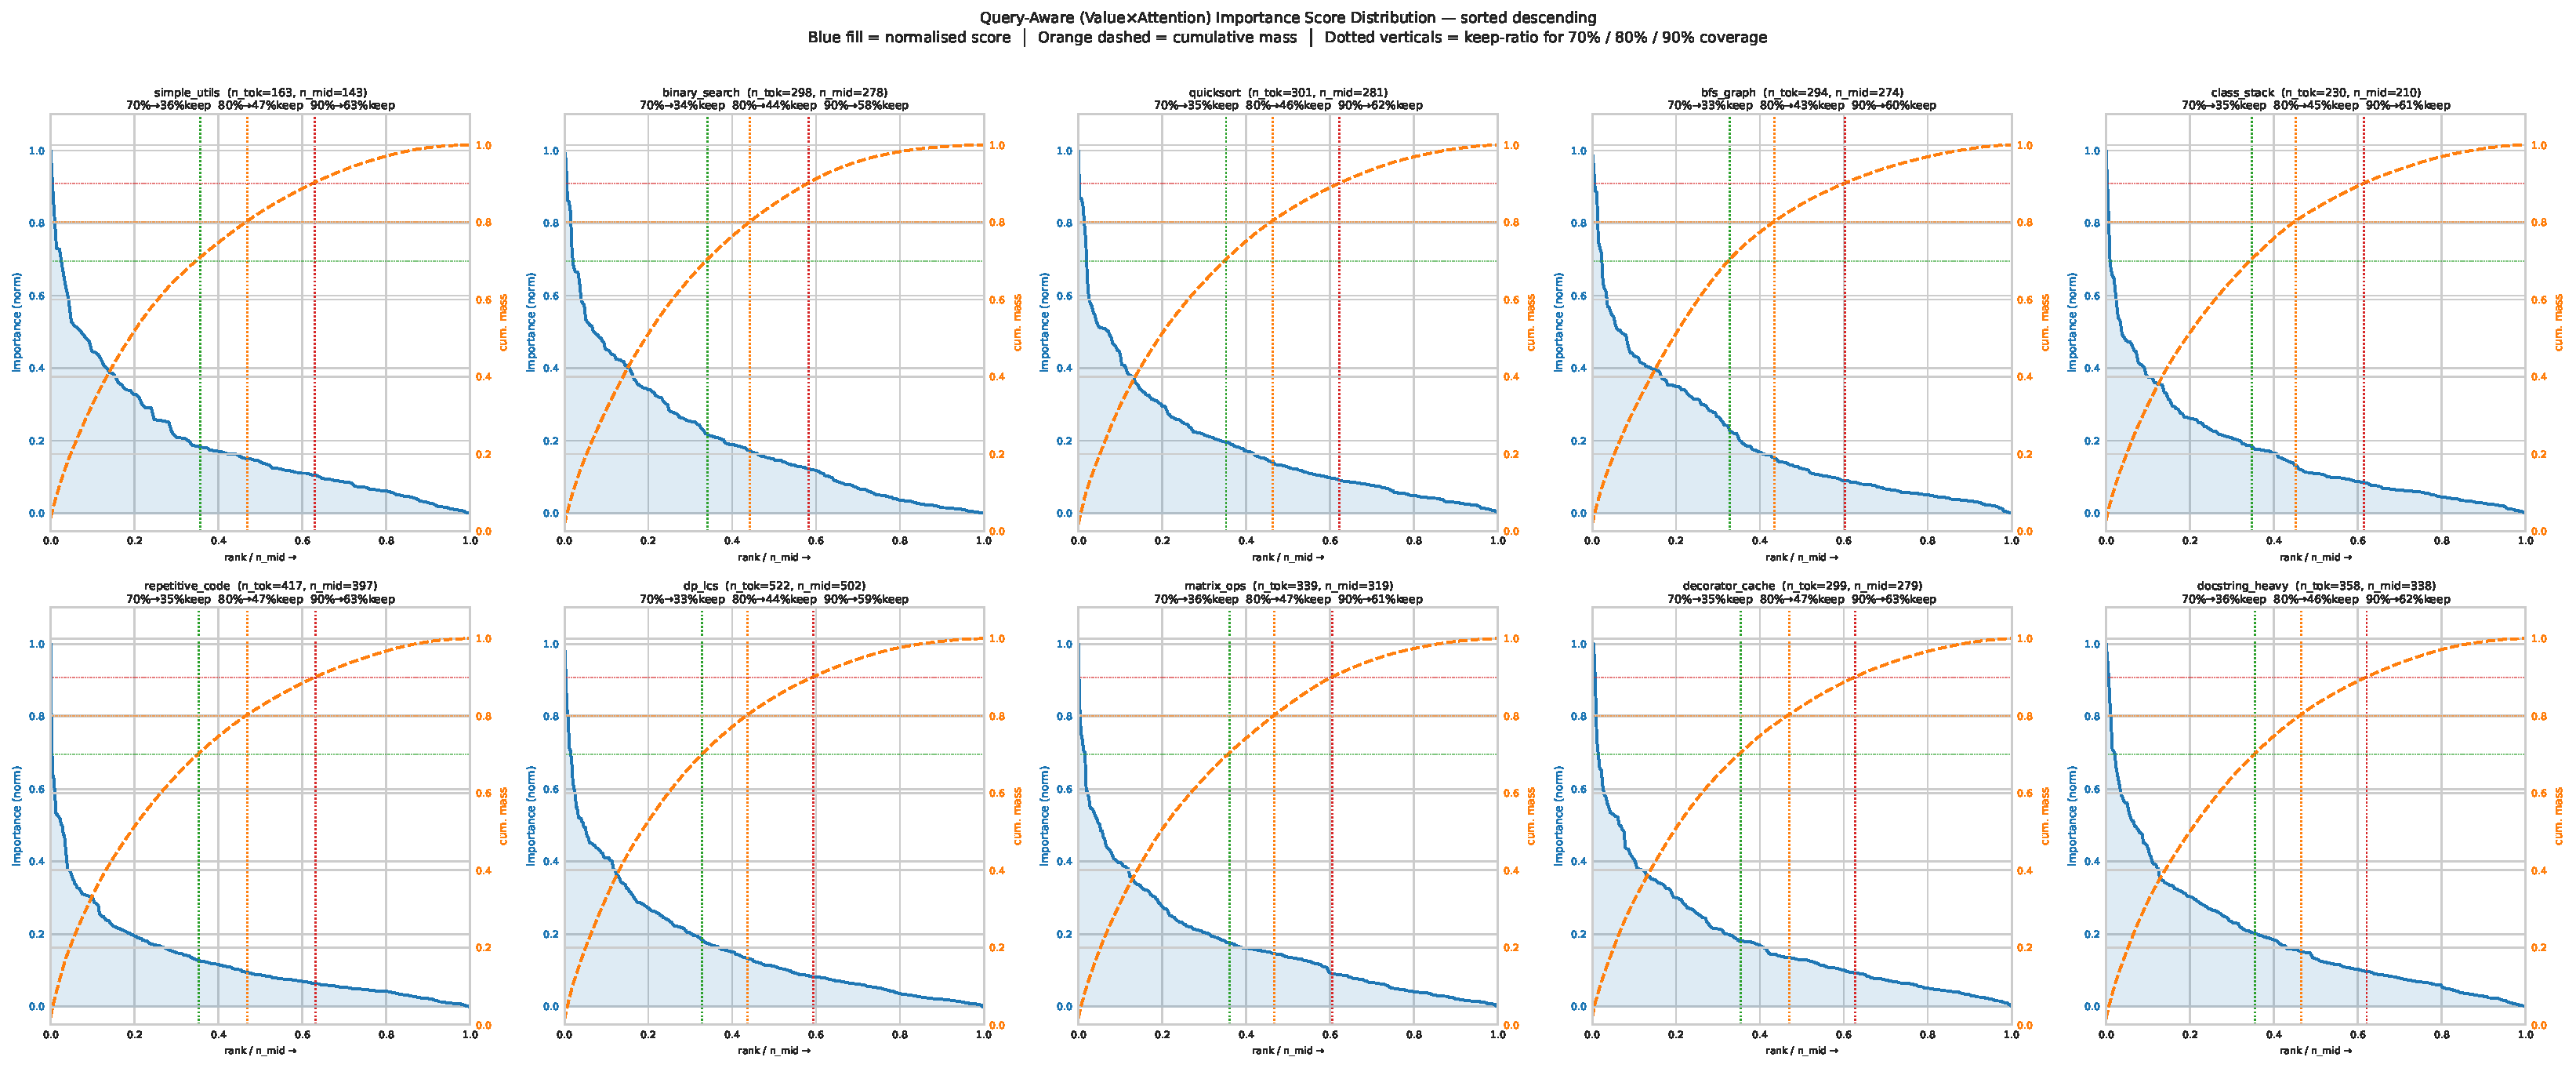
\includegraphics[width=\linewidth]{Figures/score_distributions.pdf}
  \caption{%
    Importance score distributions of latent KV vectors $\mathbf{c}^{KV}$
    profiled on code corpora. Each sub-figure shows sorted importance scores
    (blue, left axis) and the corresponding cumulative mass curve $C(k)$
    (orange dashed, right axis) for a representative sequence.
    The distributions consistently exhibit an \emph{L-shaped long-tail decay}:
    a small token minority captures the majority of importance mass, while the
    bulk of tokens are near-redundant.
    Vertical dotted lines mark the knee point $k_{\mathrm{knee}}$
    (Eq.~\ref{eq:knee}) and the coverage-floor threshold $k_{\mathrm{cov}}$
    (Eq.~\ref{eq:cov}); the adaptive budget $k^{\star}$ (Eq.~\ref{eq:budget})
    is the larger of the two.%
  }
  \label{fig:importance_dist}
\end{figure*}


\paragraph{Cumulative Mass Curve and Knee Point.}
Given the mid-token importance scores $\{\mathcal{I}[j]\}_{j=1}^{n}$,
we shift them to non-negative values and normalise to obtain a probability
mass distribution
$m[j] = \mathcal{I}[j]\,/\,\sum_k \mathcal{I}[k]$.
Sorting in descending order yields the concave cumulative-mass curve
$C(k) = \sum_{i=1}^{k} m_{(i)}$,
where $m_{(i)}$ is the $i$-th largest mass.
The \emph{knee point} of $C(k)$ is defined as the index furthest above
the diagonal $(0,0)\!\to\!(1,1)$:
\begin{equation}
  k_{\mathrm{knee}}
  = \arg\max_{k}\!\left[C(k) - \frac{k}{n}\right].
  \label{eq:knee}
\end{equation}
Geometrically, $C(k)-k/n$ measures the vertical distance from the
diagonal to the curve.
A concentrated importance distribution produces a steep early $C(k)$,
placing the knee at a small $k_{\mathrm{knee}}$ and permitting aggressive
eviction. A near-uniform distribution produces a shallow curve, yielding a
larger $k_{\mathrm{knee}}$ and mandating conservative retention.
The knee criterion thus adapts the budget to the content of each sequence
without any learned threshold.

\paragraph{Coverage Floor.}
Knee detection alone can under-retain tokens when the distribution is
approximately uniform---the knee settles near $n/2$, discarding tokens that
collectively carry non-negligible importance mass. We therefore impose a
\emph{coverage floor} $\tau$ (default $0.85$) that guarantees a minimum
retained mass fraction:
\begin{equation}
  k_{\mathrm{cov}}
  = \min\, k \;\;\text{s.t.}\;\; C(k) \geq \tau.
  \label{eq:cov}
\end{equation}

\paragraph{Final Adaptive Budget.}
The two estimates are combined as
\begin{equation}
  k^{\star}
  = \operatorname{clamp}\!\Bigl(
      \max\!\bigl(k_{\mathrm{knee}},\;k_{\mathrm{cov}}\bigr),\;
      \lceil\rho_{\min} n\rceil,\;
      \lfloor\rho_{\max} n\rfloor
    \Bigr),
  \label{eq:budget}
\end{equation}
where $\rho_{\min}$ and $\rho_{\max}$ are hard ratio bounds
(defaults $0.30$ and $0.98$).
Taking the maximum of the two estimates ensures that neither the
shape-adaptive signal nor the mass-coverage guarantee is sacrificed:
if the knee is overly conservative, the coverage floor tightens the budget;
if the knee is overly aggressive, the coverage floor prevents excessive
information loss.
This formulation requires no trainable parameters and introduces negligible
overhead---sorting $n$ scores is $\mathcal{O}(n\log n)$, dominated by the
$\mathcal{O}(HKn)$ importance-scoring step.

\subsection{Soft Eviction via Super Tokens}

Hard eviction---permanently discarding low-ranked tokens from the cache---is
irreversible: information carried by evicted tokens is lost to all subsequent
decoding steps. This is particularly damaging for long-range retrieval tasks,
where a token that appears informationally marginal during prefill may become
highly relevant hundreds of positions later~\cite{xiao2024streamingllm}.

\paragraph{Super-Token Construction.}
Rather than discarding evicted mid-tokens, CalveKV \emph{merges} them into
compact \emph{super tokens} that are appended to the end of the KV cache.
Consecutive evicted tokens are grouped into non-overlapping chunks of size
$\rho_p$ (pool ratio, default $4$), and each chunk is reduced to a single
super token via two complementary pooling strategies applied to the two
components of the latent cache.

\emph{Content pooling} (latent vector $\mathbf{c}$).
Tokens within a chunk are combined via an importance-score-weighted softmax
average:
\begin{equation}
  \mathbf{c}_{\mathrm{super}}
  = \sum_{t\in\mathrm{chunk}}
    \operatorname{softmax}\!\!\left(\frac{\mathcal{I}(t)}{T}\right)
    \mathbf{c}_{t},
  \quad T = 0.1,
  \label{eq:super_c}
\end{equation}
where $T$ is a sharpness temperature. A low $T$ concentrates weight on the
highest-scored token within the chunk, preserving its dominant latent signal;
higher $T$ approaches a uniform average over the chunk.

\emph{Position pooling} (RoPE key $\mathbf{k}^{R}$).
Positional components are averaged uniformly:
\begin{equation}
  \mathbf{k}^{R}_{\mathrm{super}}
  = \frac{1}{\rho_p}\sum_{t\in\mathrm{chunk}} \mathbf{k}^{R}_{t}.
  \label{eq:super_kpe}
\end{equation}
Importance weighting is intentionally \emph{not} applied to positional
components: RoPE encodes absolute positions through phase rotations in the
complex plane, and a biased phase average would distort the rotary coherence
required for correct positional interpolation during decoding. Uniform averaging
preserves spatial locality while producing a valid positional representation
for the merged chunk.

\paragraph{Cache Layout and Compression Benefit.}
After eviction and merging, the physical KV cache for each layer is laid out as:
\begin{equation}
  \underbrace{[\,\text{sink} \;\|\; \text{kept-mid} \;\|\; \text{recent}\,]}_{\text{preserved tokens}}
  \;\Bigl\|\;
  \underbrace{[\,\mathbf{c}^{\mathrm{super}}_{1},\,\ldots,\,
               \mathbf{c}^{\mathrm{super}}_{n_s}\,]}_{\text{super tokens}},
  \label{eq:cache_layout}
\end{equation}
where $n_s = \lfloor n_{\mathrm{evicted}}/\rho_p \rfloor$.
The protected sink and recency regions remain unmodified.
Super tokens are treated as ordinary cache entries during autoregressive
decoding---no special attention masking or retrieval mechanism is required,
and the attention computation path is entirely unchanged.
The net effect is an additional $\rho_p$-fold reduction in the memory
footprint of evicted tokens:
$n_{\mathrm{evicted}}$ tokens are replaced by $n_{\mathrm{evicted}}/\rho_p$
super tokens, achieving further compression beyond the primary eviction step
without permanently discarding any prefill context.








\section{Experiments}


\subsection{Experimental Setup}

\paragraph{Model and Hardware.}
All experiments are conducted on DeepSeek-Coder-V2-Lite~\cite{deepseekv2},
a 16-billion-parameter MLA-based code language model supporting a 128K-token
context window and employing a 27-layer Transformer backbone with
$d_c = 512$ KV latent rank.
All inference runs are performed on a single NVIDIA GPU with 48\,GB of device
memory under PyTorch 2.3.0 and CUDA 12.1.
No model weights are modified; CalveKV operates purely at the inference level.

\paragraph{Compared Configurations.}
We evaluate the following configurations.
\texttt{baseline}: standard MLA inference with no eviction.
\texttt{committee\_c85} / \texttt{committee\_c90}: the full CalveKV pipeline
with multi-layer committee scoring ($\mathcal{S}=\{4,6,8,12,16\}$),
adaptive budget at coverage floor $\tau=0.85$ / $\tau=0.90$, and
soft eviction via super-token pooling ($\rho_p=4$).
\texttt{hard\_evict\_c90}: committee scoring with $\tau=0.90$ but
\emph{hard} eviction (no super-token aggregation), isolating the
contribution of soft eviction.
\texttt{single\_L6} / \texttt{single\_L12}: single-layer eviction using
only the L6 or L12 score, with adaptive budget ($\tau=0.90$) and soft
eviction, isolating the benefit of committee voting.
\texttt{fixed\_ratio\_70}: a non-adaptive baseline that retains a fixed
70\% of mid-range tokens regardless of the importance distribution,
isolating the contribution of the adaptive budget mechanism.

\paragraph{Evaluation Dimensions.}
Our evaluation covers five complementary dimensions.
(1)~\emph{Cross-layer persistence} (Section~\ref{sec:exp_persistence}):
Spearman rank correlation and Jaccard keep-set overlap across ten
candidate layers, directly validating the foundational assumption of
committee-based shared eviction.
(2)~\emph{Language modelling quality} (Section~\ref{sec:exp_suffix_ppl}):
Suffix perplexity on \texttt{code-search-net/python}, measuring how well
the post-eviction cache supports continuation.
(3)~\emph{Long-context retrieval} (Section~\ref{sec:exp_niah}):
multi-needle NIAH recall at context lengths of 2k and 4k tokens.
(4)~\emph{Code structural understanding}
(Sections~\ref{sec:exp_code_recall} and~\ref{sec:exp_humaneval}):
cross-reference recall across six symbol types and HumanEval
syntax-pass@1.
(5)~\emph{System efficiency} (Section~\ref{sec:exp_system}):
KV cache compression ratio, prefill latency, Time-to-First-Token (TTFT),
and peak VRAM consumption across context lengths from 1k to 12k tokens.



\subsection{Cross-Layer Importance Persistence Analysis}
\label{sec:exp_persistence}

The multi-layer committee design assumes that importance scores of a latent from an
early layer reliably predict which tokens matter in later layers.
We test this directly across ten layers of the 27-layer backbone:
$\{$L0, L1, L2, L4, L6, L8, L10, L12, L16, L20$\}$.

\paragraph{Setup.}
For each test sequence, all ten layers are instrumented simultaneously
via forward hooks and the full $\mathcal{I}^{(\ell)}[j]$ score vector
(Eq.~\eqref{eq:importance}) is computed at every layer in a single
forward pass.
The same query subsample (Eq.~\eqref{eq:sampled}) is shared across all
layers to remove Monte Carlo variance from the comparison.
Two metrics quantify cross-layer consistency.

\emph{Spearman rank correlation $\rho(\ell_1,\ell_2)$} measures whether
the importance ordering at $\ell_1$ is preserved at $\ell_2$, averaged
over all test sequences.

\emph{Jaccard keep-set overlap $J(\ell_1,\ell_2)$} is the Jaccard index
of the top-30\% keep sets selected independently at each layer:
\begin{equation}
  J(\ell_1,\ell_2)
  = \frac{|\mathcal{K}^{(\ell_1)}\cap\mathcal{K}^{(\ell_2)}|}
         {|\mathcal{K}^{(\ell_1)}\cup\mathcal{K}^{(\ell_2)}|}.
\end{equation}
This directly measures whether two layers would reach the same eviction
decision.


Figure~\ref{fig:cross_layer_corr} presents the $10\times10$ matrices.

Layers L0--L2 show substantially lower agreement with later layers than
layers in the L4--L20 block, matching the elevated PPL in
Table~\ref{tab:gap_vs_oracle} when those layers are used as sole
decision-makers (PPL $= 26.58$, $13.82$, $15.42$ at L0, L1, L2).

From L4 onward, all pairwise Spearman correlations exceed $\rho > 0.84$.
Adjacent layers reach $\rho \approx 0.96$ (e.g.\ L4--L6, L6--L8).
The Jaccard results follow the same pattern: L4 and L6 share $J = 0.81$
of their keep sets, falling to $J = 0.66$ at the widest gap tested
(L4 vs.\ L16), still well above the chance baseline of $J = 0.43$.

\begin{figure}[t]
  \centering
  \begin{minipage}[t]{0.485\linewidth}
    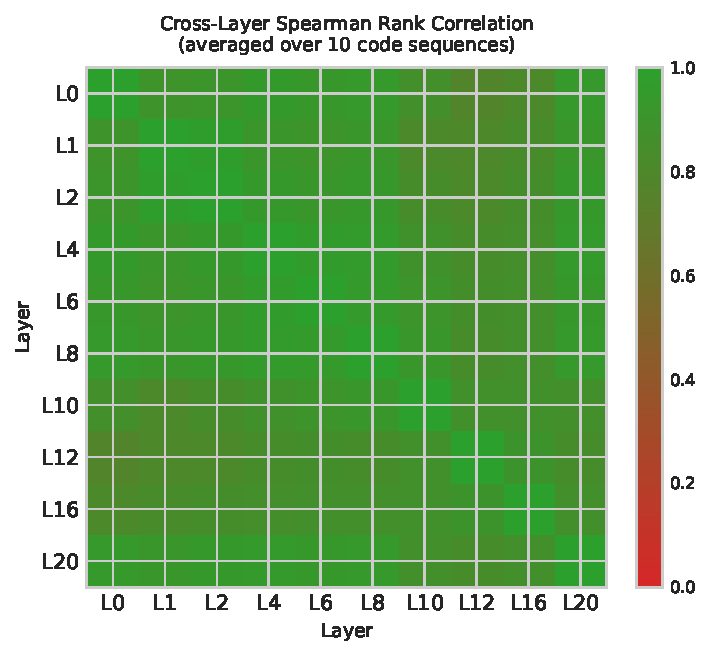
\includegraphics[width=\linewidth]{Figures/cross_layer_correlation.pdf}
  \end{minipage}
  \hfill
  \begin{minipage}[t]{0.485\linewidth}
    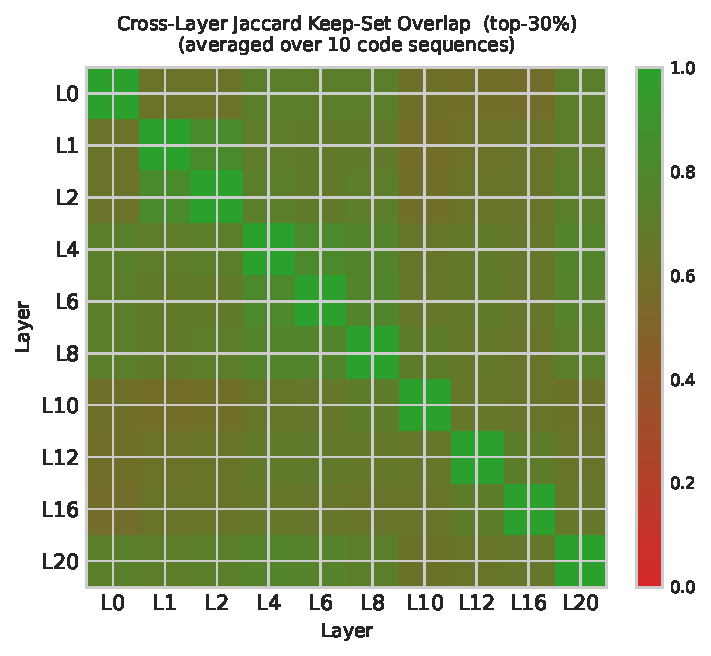
\includegraphics[width=\linewidth]{Figures/cross_layer_jaccard.pdf}
  \end{minipage}
  \caption{%
    Cross-layer importance consistency across ten layers, averaged over
    ten code sequences.
    \emph{Left}: Spearman rank correlation $\rho$.
    \emph{Right}: Jaccard overlap of the top-30\% keep sets.
    Green = high agreement; red = low agreement.%
  }
  \label{fig:cross_layer_corr}
\end{figure}


Figure~\ref{fig:trajectory} tracks individual tokens across all ten
layers for three sequences: \texttt{quicksort} (concentrated
distribution), \texttt{binary\_search} (moderate), and
\texttt{repetitive\_code} (near-uniform).
For each sequence, the five highest-ranked, five median-ranked, and
five lowest-ranked mid-tokens by L4 score are followed through all
ten layers.

High-importance tokens (red) stay above the 90th percentile from L4 to
L20 in all three sequences.
Low-importance tokens (blue) remain near zero throughout.
Mid-importance tokens (grey) fluctuate between layers; per-layer scoring
noise concentrates in this ambiguous middle tier rather than at the
extremes that govern the eviction boundary.

Kendall correlations between L4 and the other committee layers range
from $\tau = 0.63$ at L12 to $\tau = 0.87$ at L6.

\begin{figure*}[t]
  \centering
  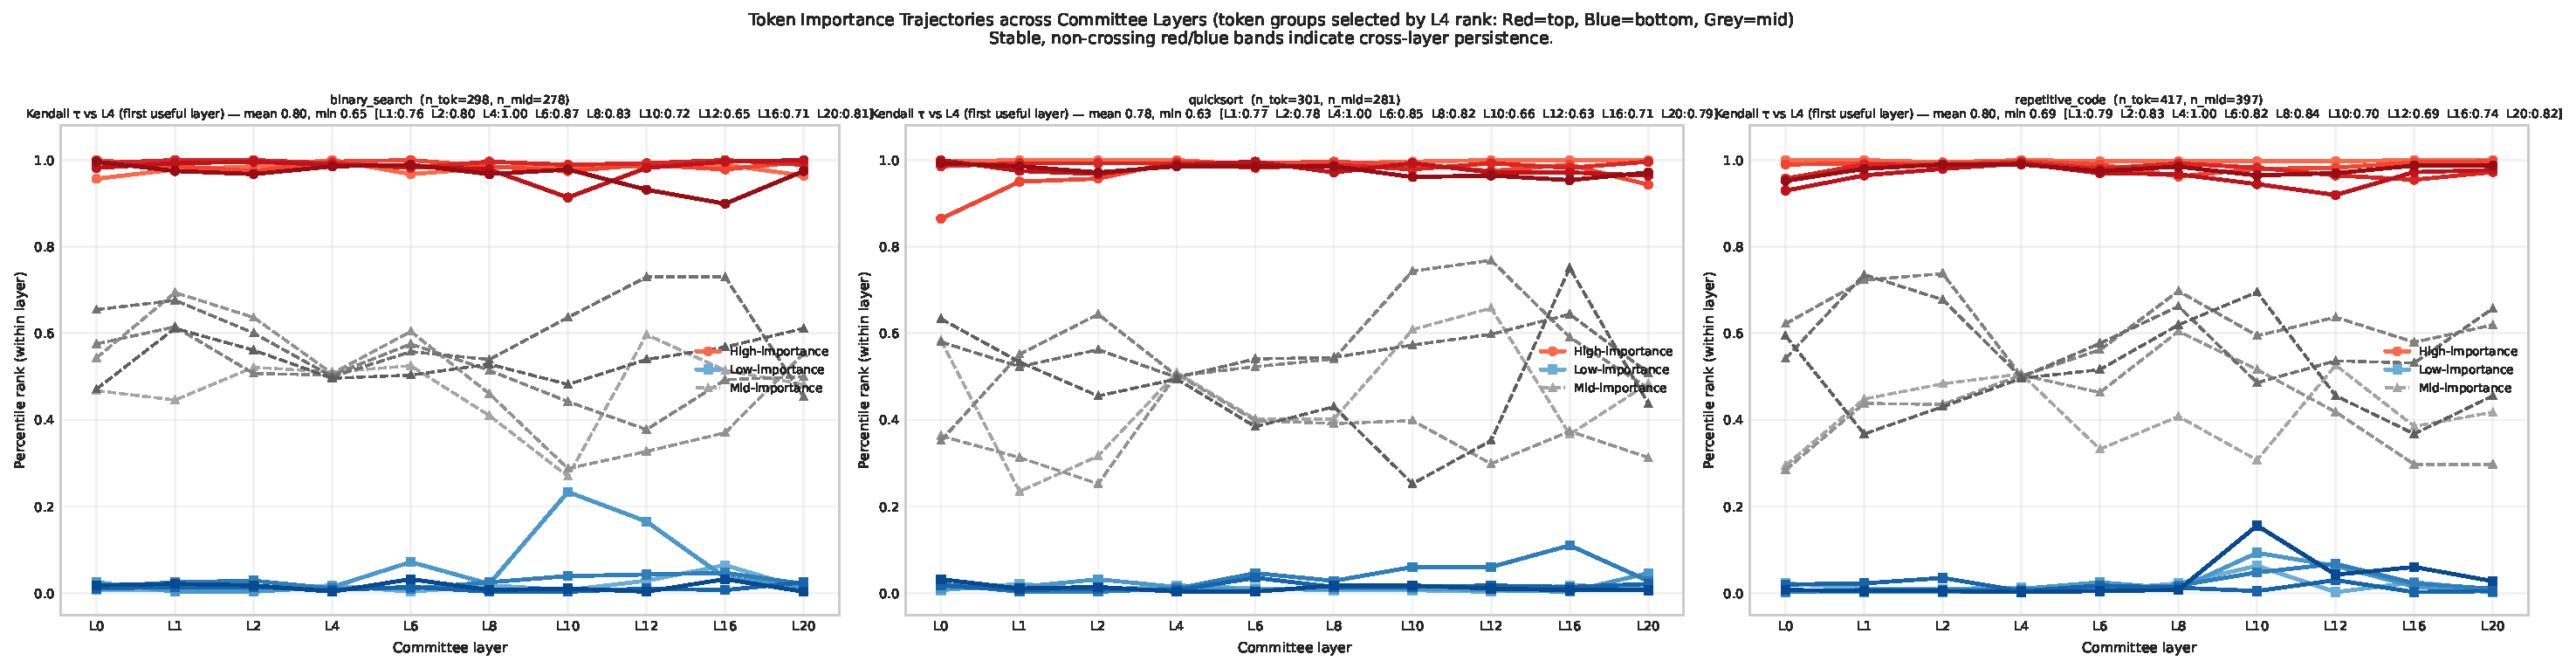
\includegraphics[width=\linewidth]{Figures/trajectory_combined.pdf}
  \caption{%
    Per-token importance trajectories across ten layers for three code
    sequences.
    Token groups are defined by L4 percentile rank:
    red $=$ top-5, blue $=$ bottom-5, grey $=$ middle-5.
    The $y$-axis shows within-layer percentile rank at each layer
    (0 = least important, 1 = most important).%
  }
  \label{fig:trajectory}
\end{figure*}


We see that L0--L2 are clearly unsuitable as scoring sources.
Within the L4--L20 block, L12 shows the largest deviation from L4
($\tau = 0.63$), confirming that no single layer generalises perfectly
across all others.
Averaging over $\mathcal{S} = \{4,6,8,12,16\}$ reduces per-layer noise
and yields a more stable consensus ranking, consistent with
\texttt{committee\_c85} achieving the lowest Suffix PPL among all
eviction strategies (Table~\ref{tab:suffix_ppl}).






\subsection{Suffix PPL test}

\label{sec:exp_suffix_ppl}


Suffix PPL evaluates how much generation quality is preserved after cache eviction.
For each sample, we first run a \emph{prefix prefill} pass, eviction may be triggered,
then we compute the negative log-likelihood (NLL) on the following suffix tokens conditioned on
the post-eviction KV cache.
Formally, for suffix tokens $\mathbf{y}_{1:T}$:
\begin{equation}
\mathrm{NLL} = -\frac{1}{T}\sum_{t=1}^{T}\log p(y_t \mid \mathbf{x}_{\mathrm{prefix}}, \mathbf{y}_{<t}; \,\text{post-eviction cache}),
\end{equation}
\begin{equation}
\mathrm{Suffix\ PPL} = \exp(\mathrm{NLL}).
\end{equation}
Lower Suffix PPL indicates less quality degradation under the same cache budget strategy.


We use \texttt{code-search-net/python} as the evaluation corpus (12,928 tokens), with
$n=20$ samples. This metric directly tests whether the evicted cache still preserves
useful predictive information for continuation. It shows whether the LLM can "speak" normally.
Table 2 shows the experiments result.

\begin{table}[t]
\centering
\small
\caption{Suffix PPL on \texttt{code-search-net/python} (lower is better).}
\label{tab:suffix_ppl}
\begin{tabular}{lr}
\toprule
Configuration & Suffix PPL \\
\midrule
baseline          & 2.546 \\
committee\_c85    & 3.571 \\
committee\_c90    & 3.611 \\
single\_L6        & 3.621 \\
fixed\_ratio\_70  & 3.919 \\
hard\_evict\_c90  & 4.066 \\
single\_L12       & 4.129 \\
\bottomrule
\end{tabular}
\end{table}

Compared with baseline, all eviction variants increase Suffix PPL, this proves the expected
quality--compression trade-off.
Among eviction methods, \texttt{committee\_c85} achieves the best PPL (3.571).
\texttt{committee\_c90} and \texttt{single\_L6} are very close (3.611/3.621), suggesting
that multi-layer committee scoring is robust and competitive in this setting.
\texttt{hard\_evict\_c90} is clearly worse than \texttt{committee\_c90} (4.066 vs 3.611),
indicating that soft-eviction/super-token aggregation helps recover predictive information.
\texttt{fixed\_ratio\_70} underperforms adaptive committee variants, supporting the value of
adaptive budgeting over a rigid keep ratio.
Finally, \texttt{single\_L12} is the weakest among tested eviction strategies (4.129),
suggesting that relying on a single deeper layer is less stable than committee or L6-based decisions.

\subsection{Needle-in-a-Haystack (NIAH) Evaluation}
\label{sec:exp_niah}

Needle-in-a-Haystack (NIAH) can evaluate long-context retrieval fidelity under cache eviction.
In standard NIAH tests, both the baseline and all configurations achieve (100\%) recall.
So we employ a \emph{multi-needle setup} to increase discrimination: a target integer constant is
marked as ``REAL ANSWER'' and surrounded by 5 randomly-generated decoy constants
(CACHE\_SIZE, BUFFER\_LENGTH, MAX\_RETRIES, TIMEOUT\_MS, VERSION).
The model is instructed to ignore decoys and only return the value of the 
real constant. Strict output matching is enforced: answers without an ``Answer:'' 
prefix or embedded within variable names are rejected.
This challenging variant reveals fine-grained quality differences across eviction strategies.
But naive NIAH setups may miss.

\begin{table}[t]
\centering
\small
\caption{NIAH recall (\%) at different context lengths under multi-needle protocol. Higher is better.}
\label{tab:niah_main}
\begin{tabular}{lccc}
\toprule
Context Length & baseline & committee\_c90 & committee\_c85 \\
\midrule
2048 & 67\% & 67\% & 83\% \\
4096 & 0\% & 33\% & 33\% \\
\bottomrule
\end{tabular}
\end{table}

The multi-needle NIAH results reveal substantial performance gaps not visible in prior
saturated benchmarks. At 2k tokens, \texttt{committee\_c85} achieves 83\% recall, 
outperforming the baseline (67\%) and \texttt{committee\_c90} (67\%).
The gap widens at 4k tokens: both committee variants sustain 33\% recall, while
the no-eviction baseline drops to 0\%, indicating systematic needle loss under eviction
pressure at longer contexts. 

These results demonstrate that our CalveKV's adaptive budget and soft-eviction mechanisms
provide meaningful protection for long-range retrieval, even under increased difficulty.
Unlike prior NIAH evaluations that reported near-perfect recall, the multi-needle 
protocol with strict output matching serves as a genuinely discriminative benchmark
for eviction-induced degradation across context lengths.

Additionally, we ablate the soft-eviction component, we can see the result in table 4:

\begin{table}[t]
\centering
\small
\caption{Ablation: soft eviction impact on NIAH recall (\%).}
\label{tab:niah_ablation}
\begin{tabular}{lcc}
\toprule
Configuration & ctx=2k & ctx=4k \\
\midrule
committee\_hard\_c90 (no super-tokens) & 100\% & 17\% \\
committee\_c90 (with super-tokens) & 67\% & 33\% \\
\bottomrule
\end{tabular}
\end{table}

Interestingly, hard eviction performs better at 2k (100\% vs 67\%), suggesting that at moderate 
context lengths, information loss from 
discarding is less harmful than the noise introduced by approximate super-token pooling.
However, at 4k the trend reverses: soft eviction (33\%) substantially outperforms 
hard eviction (17\%). It indicates that preserving low-rank residual information becomes 
critical for maintaining long-range retrieval at scale.





\subsection{Code Cross-Reference Recall}
\label{sec:exp_code_recall}

Code cross-reference recall evaluates the model's ability to retrieve variable, function, and class names 
defined far earlier in the context. This test complements the NIAH test.
It measures long-range dependency tracking in realistic code patterns rather than synthetic needles.

Each test case embeds filler code (400+ lines of utility functions, class definitions, and constants) 
between the definition of a target symbol and a prompt asking the model to complete a reference to that symbol.
The test verifies whether the cached KV representations preserve sufficient information for 
accurate recall. We conducted experiments across the following dimensions:

\begin{itemize}
  \item \emph{Class constant}: Reference to a constant defined within a class (\texttt{Config.DATABASE\_POOL\_SIZE})
  \item \emph{Module secret}: Reference to a module-level variable (\texttt{ENCRYPTION\_KEY})
  \item \emph{Function recall}: Call to a user-defined function (\texttt{validate\_email()})
  \item \emph{Dataclass field}: Access to a field from a dataclass (\texttt{cfg.learning\_rate})
  \item \emph{Exception class}: Reference to a custom exception type (\texttt{ConnectionTimeoutError})
  \item \emph{Protocol constant}: Reference to a protocol-level constant (\texttt{MAGIC\_HEADER})
\end{itemize}

\begin{table*}[t]
\centering
\small
\caption{Code cross-reference recall (\%) by symbol type. Higher is better.}
\label{tab:code_recall}
\begin{tabular}{lccccccc}
\toprule
Configuration & Class & Module & Function & Dataclass & Exception & Protocol & Overall \\
 & Const & Secret & Recall & Field & Class & Const & Score \\
\midrule
baseline & \checkmark & \checkmark & -- & -- & -- & \checkmark & 50\% \\
committee\_c90 & \checkmark & \checkmark & \checkmark & -- & -- & \checkmark & 67\% \\
committee\_c85 & \checkmark & \checkmark & \checkmark & -- & -- & \checkmark & 67\% \\
hard\_evict\_c90 & \checkmark & \checkmark & \checkmark & -- & -- & \checkmark & 67\% \\
fixed\_ratio\_70 & \checkmark & \checkmark & \checkmark & -- & -- & \checkmark & 67\% \\
single\_L6 & \checkmark & \checkmark & \checkmark & -- & -- & \checkmark & 67\% \\
single\_L12 & \checkmark & \checkmark & -- & -- & -- & \checkmark & 50\% \\
\bottomrule
\end{tabular}
\end{table*}


Results is shown in table 5. We observed that the eviction committee variants (\texttt{committee\_c90}, \texttt{hard\_evict\_c90}, \texttt{fixed\_ratio\_70}, \texttt{single\_L6}) 
uniformly achieve 67\% recall, successfully preserving four of six symbol types. Notably, all configurations fail on 
\emph{dataclass field} and \emph{exception class} retrieval, including the baseline. It suggests that these require finer-grained type information 
that may be systematically under-represented in the eviction scoring.

The baseline achieves only 50\% recall, failing on both function recall and exception classes, 
despite having access to the full KV cache. This indicates that naive full-cache retention does not guarantee 
long-range dependency fidelity. The model still loses track of certain symbol definitions under long context.

Interestingly, \texttt{single\_L12} (relying on a single deeper layer for importance scoring) drops to 50\%, 
matching the baseline. This suggests that deeper layers alone provide insufficient signal for preserving 
syntactic anchors, such as function names or exception types. These are critical for code structure understanding. 
The multi-layer committee's superior performance (67\%) demonstrates that blending importance estimates 
from shallow, intermediate, and deep layers better preserves the diverse semantic and syntactic information 
needed for cross-reference resolution.

The uniformity of recall patterns across eviction strategies (committee, hard eviction, fixed ratio, single layers) 
at 67\% suggests that the failures on dataclass fields and exception classes reflect limitations in the underlying 
importance-scoring formulation rather than eviction-specific degradation. This points to a direction for future work: 
enriching the scoring function to better capture type-definition information.



%%考虑要不要删掉，因为这是负面的-----------------------------------------------------------------------------
\subsection{HumanEval Syntax-Pass@1}
\label{sec:exp_humaneval}

HumanEval syntax-pass@1 evaluates whether the model can generate syntactically valid Python code
given a function signature and docstring. Unlike full functional correctness, this metric focuses
solely on whether the generated output is parseable by the Python interpreter---a necessary
precondition for any downstream execution or testing. We sample one completion per problem
and report the fraction of outputs that pass \texttt{ast.parse()} without errors, using a
20-problem subset drawn from the 164-problem HumanEval benchmark~\cite{chen2021humaneval}.

\begin{table}[t]
\centering
\small
\caption{HumanEval syntax-pass@1 (\%) on a 20-problem subset. Higher is better.}
\label{tab:humaneval}
\begin{tabular}{lcc}
\toprule
Configuration & Pass Count & Syntax-Pass@1 \\
\midrule
baseline         & 14/20 & 70\% \\
committee\_c90   &  8/20 & 40\% \\
hard\_evict\_c90 &  8/20 & 40\% \\
fixed\_ratio\_70 &  9/20 & 45\% \\
single\_L6       &  7/20 & 35\% \\
single\_L12      &  9/20 & 45\% \\
\bottomrule
\end{tabular}
\end{table}

The baseline achieves 70\% syntax-pass@1, substantially outperforming all eviction
variants, which cluster between 35--45\%. This gap reflects an inherent tension between
cache compression and generative coherence: KV eviction during prefill discards context
that the model relies on to maintain syntactic structure across multi-line code generation.

Among eviction strategies, \texttt{fixed\_ratio\_70} and \texttt{single\_L12} tie at 45\%,
narrowly ahead of \texttt{committee\_c90} and \texttt{hard\_evict\_c90} (both 40\%), while
\texttt{single\_L6} falls lowest at 35\%. Notably, the committee-based soft eviction does
not provide a clear advantage over hard eviction on this metric---both yield 40\%---
suggesting that super-token pooling, while beneficial for retrieval tasks (Section~\ref{sec:exp_niah}),
does not recover syntactic generation quality lost through latent compression.

The overall degradation across all eviction variants indicates that code generation tasks,
which require maintaining open syntactic structures (function bodies, indentation blocks,
return statements) over hundreds of tokens, are more sensitive to context loss than
retrieval tasks. This motivates future work on selectively protecting generation-critical
context during the eviction phase.

%%----------------------------------------------------------------------------------------------



\subsection{System Metrics}
\label{sec:exp_system}

To characterize the computational and memory efficiency of CalveKV under realistic
conditions, we conduct a systematic profiling study across a range of context lengths
($\{1024, 2048, 4096, 6144, 8192, 12288\}$ tokens). Due to the limitation of our laboratory, 
the maximum context is 12k in our test, but it is enough to prove the effectness of CalveKV.
For each configuration, we measure
four indicators: (i) \emph{KV compression ratio}, defined as the fraction of latent cache
entries retained after eviction relative to the full cache; (ii) \emph{prefill latency}
(ms), the wall-clock time to process the entire input prompt; (iii)
\emph{Time-to-First-Token} (TTFT, ms), the latency from prompt completion to the emission
of the first generated token; and (iv) \emph{peak VRAM consumption} (GB), recorded at the
end of the prefill phase. All experiments are conducted on a single NVIDIA GPU with 48 GB
of device memory under PyTorch 2.3.0 and CUDA 12.1. We have thre configuration compaerd with
baseline.

\begin{table*}[t]
\centering
\small
\caption{System metrics across context lengths. Compress = retained KV fraction (\%);
Prefill = prefill latency (ms); TTFT = time-to-first-token (ms);
VRAM = peak GPU memory (GB). Lower is better for Prefill, TTFT, and VRAM.}
\label{tab:system_metrics}
\begin{tabular}{llrrrr}
\toprule
Configuration & Context & Compress & Prefill & TTFT & VRAM \\
              & (tokens) & (\%) & (ms) & (ms) & (GB) \\
\midrule
baseline            & 1024  & 100.0 & 415  & 77.0 & 30.64 \\
baseline            & 2048  & 100.0 & 276  & 57.0 & 30.63 \\
baseline            & 4096  & 100.0 & 486  & 57.2 & 33.19 \\
baseline            & 6144  & 100.0 & 815  & 62.0 & 37.75 \\
baseline            & 8192  & 100.0 & 1185 & 56.8 & 44.08 \\
baseline            & 12288 & 100.0 & 2421 & 56.7 & 62.05 \\
\midrule
\texttt{committee\_c90}  & 1024  & 69.8 & 260  & 49.8 & 30.08 \\
\texttt{committee\_c90}  & 2048  & 69.1 & 272  & 48.4 & 30.69 \\
\texttt{committee\_c90}  & 4096  & 68.4 & 473  & 46.6 & 33.25 \\
\texttt{committee\_c90}  & 6144  & 68.6 & 777  & 46.4 & 37.76 \\
\texttt{committee\_c90}  & 8192  & 68.2 & 1197 & 46.5 & 44.05 \\
\texttt{committee\_c90}  & 12288 & 67.4 & 2423 & 46.5 & 61.95 \\
\midrule
\texttt{committee\_c85}  & 1024  & 64.2 & 219  & 46.9 & 30.07 \\
\texttt{committee\_c85}  & 2048  & 62.5 & 298  & 46.6 & 30.68 \\
\texttt{committee\_c85}  & 4096  & 62.4 & 483  & 47.1 & 33.22 \\
\texttt{committee\_c85}  & 6144  & 61.9 & 782  & 52.0 & 37.75 \\
\texttt{committee\_c85}  & 8192  & 62.2 & 1204 & 50.9 & 44.04 \\
\texttt{committee\_c85}  & 12288 & 61.9 & 2442 & 47.4 & 61.92 \\
\midrule
\texttt{committee\_hard\_c90} & 1024  & 59.5 & 212  & 46.9 & 30.07 \\
\texttt{committee\_hard\_c90} & 2048  & 58.4 & 275  & 56.5 & 30.68 \\
\texttt{committee\_hard\_c90} & 4096  & 58.0 & 477  & 47.2 & 33.22 \\
\texttt{committee\_hard\_c90} & 6144  & 57.7 & 779  & 51.9 & 37.74 \\
\texttt{committee\_hard\_c90} & 8192  & 57.4 & 1187 & 47.0 & 44.03 \\
\texttt{committee\_hard\_c90} & 12288 & 56.9 & 2433 & 47.4 & 61.90 \\
\bottomrule
\end{tabular}
\end{table*}

\begin{figure*}[t]
  \centering
  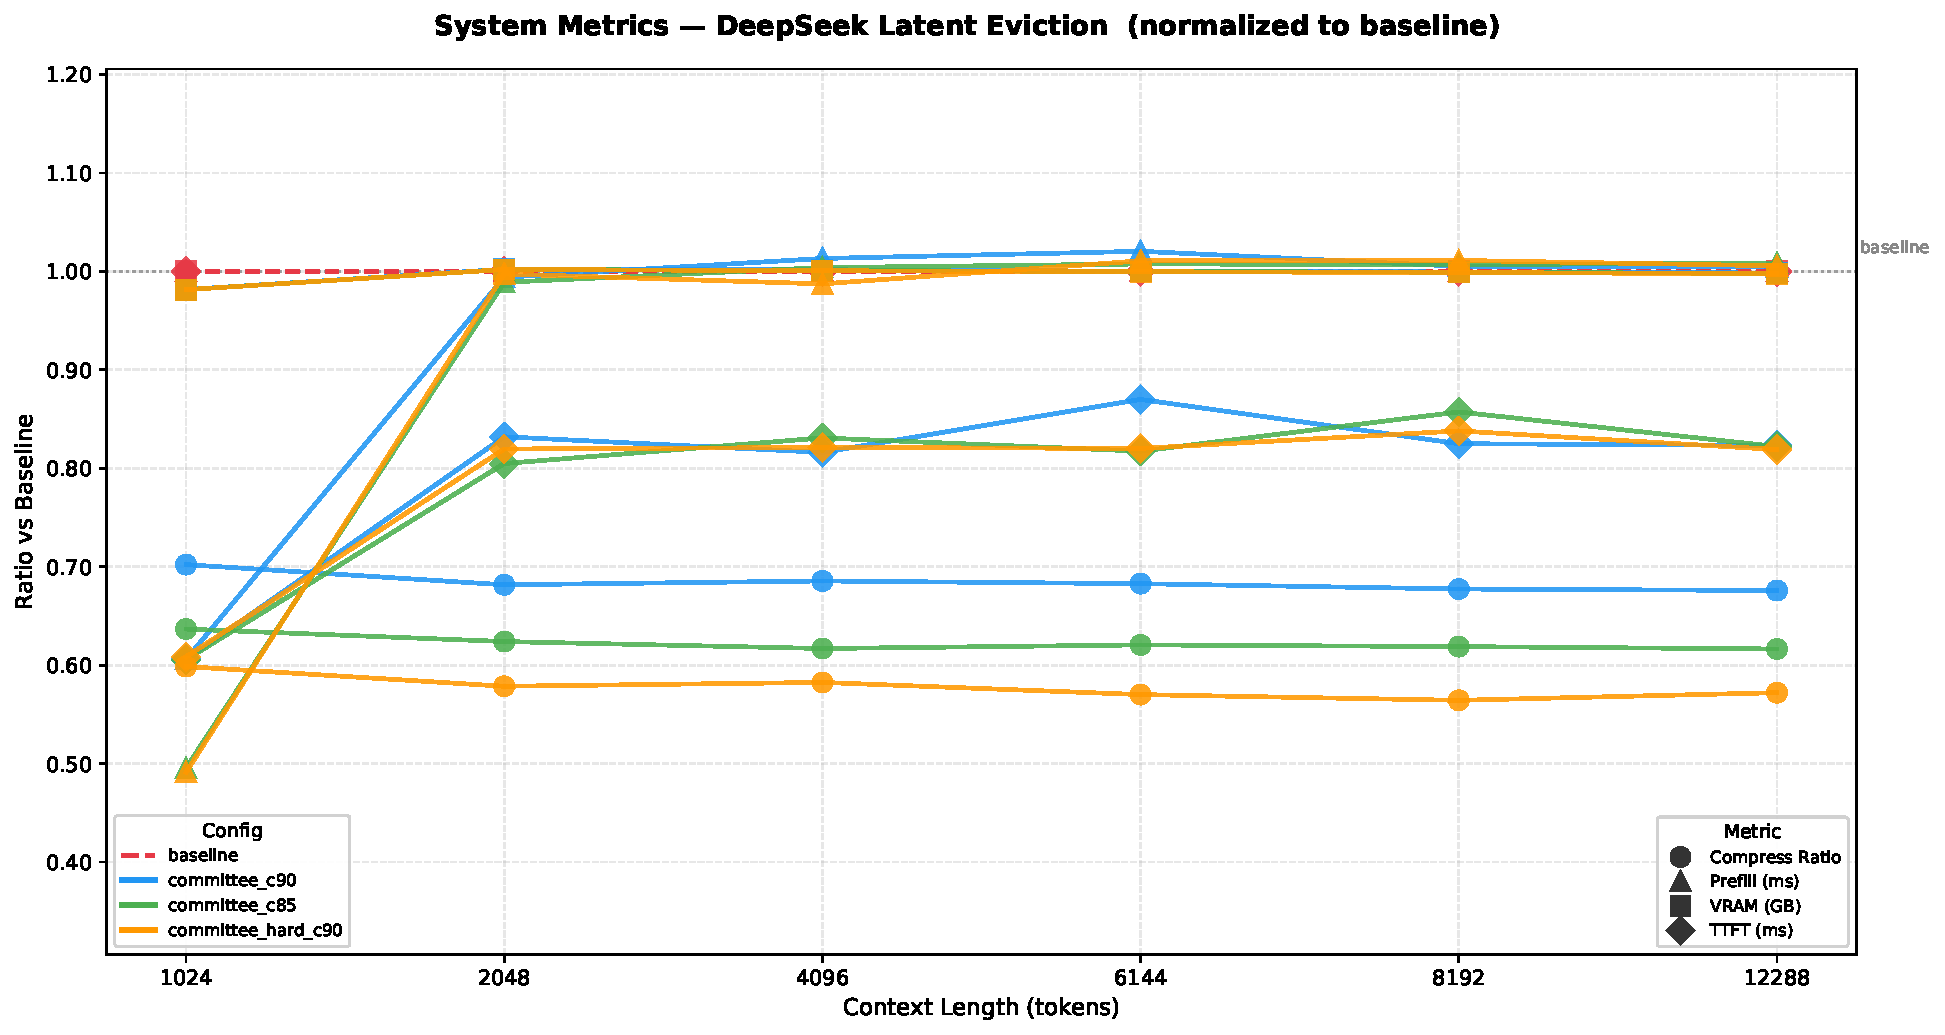
\includegraphics[width=\linewidth]{Figures/eval_results_system.pdf}
  \caption{System metrics of CalveKV variants versus the MLA baseline across context
    lengths. Top: KV cache compression ratio (\%). Middle: Time-to-First-Token (TTFT,
    ms). Bottom: peak VRAM consumption (GB).}
  \label{fig:system_metrics}
\end{figure*}

Table~\ref{tab:system_metrics} and Figure~\ref{fig:system_metrics} report the results.
We observe the following.


The compression ratio is the most direct and important indicator in the experiment.
All CalveKV variants achieve consistent compression across context lengths.
\texttt{committee\_c90} retains approximately 68--70\% of latent cache entries,
\texttt{committee\_c85} retains 62--64\%, and \texttt{committee\_hard\_c90} achieves
the most aggressive reduction at 57--60\%. Crucially, the compression ratio remains
stable as context length scales from 1k to 12k tokens. It confirms that the adaptive
budget mechanism responds consistently to the
importance distribution across diverse sequence lengths rather than exhibiting
length-dependent drift.


All CalveKV variants substantially reduce TTFT relative to the baseline.
\texttt{committee\_c90} achieves TTFT of 46--50\,ms across all context lengths,
compared to 57--77\,ms for the baseline---a reduction of approximately 20--36\%.
\texttt{committee\_c85} and \texttt{committee\_hard\_c90} exhibit comparable TTFT
profiles at 47--52\,ms. This improvement arises because the first generated token
requires a full attention sweep over all cached latent vectors, so a smaller retained
cache directly reduces this decode step. Notably, TTFT savings are consistent across
context lengths, suggesting that the eviction overhead itself is negligible relative to
the attention computation saved.


Prefill latency is broadly comparable between CalveKV variants and the baseline at
matched context lengths. We worried whether ClaveKV will increase the Prefill latency significantly,
because CalveKV performs eviction after the full prefill
attention pass, the cost of importance scoring and index selection (dominated by
the $\mathcal{O}(HKn)$ sampled attention computation with $K{=}512$ query samples). 
The test results show that CalveKV introduces no perceptible overhead at the scales tested. 
This confirms the design goal that CalveKV's eviction pipeline adds negligible computational cost 
to the prefill stage.

We observe that prefill latency is broadly comparable between CalveKV variants and the baseline at
context lengths of 2k tokens and above. Interestingly, at the context
($n{=}1024$), all CalveKV variants exhibit a substantial prefill reduction
(212--260\,ms versus 415\,ms for the baseline, a 37--49\% decrease).
We attribute this to two complementary factors.

First, the baseline figure at $n{=}1024$ is inflated by \emph{CUDA cold-start
overhead}. On the first kernel execution in each experimental run, PyTorch
incurs one-time costs for kernel compilation, CUDA context initialization, and
GPU memory-pool allocation, all of which are amortized across subsequent runs.
Because the baseline is always profiled first in our test,
it absorbs this initialization penalty disproportionately at short contexts,
where the actual compute time is otherwise negligible.

Second, CalveKV's query subsampling computes a sampled attention matrix of
shape $K \times n$ (with $K{=}512$) rather than the full $n \times n$ matrix.
At $n{=}1024$, the sampled pass requires roughly half the floating-point
operations of the standard prefill attention, and fits more favorably in L2 cache,
yielding a lower effective memory-bandwidth pressure.
At longer contexts (4k--12k), the baseline prefill time is dominated by
the $\mathcal{O}(n^2)$ attention sweep, making the $\mathcal{O}(HKn)$ scoring
overhead negligible in comparison; the two curves therefore converge.
This also confirms that CalveKV introduces no significant prefill overhead
under normal operating conditions.


Peak VRAM consumption is nearly identical across all configurations at each context
length (differences $\leq 0.15$\,GB). This is an expected result. Peak memory during prefill
is dominated by model parameters and intermediate activations rather than the KV
cache itself, whose size at the end of prefill constitutes a minor fraction of total
device memory at these context lengths. The true memory savings of CalveKV are realized during 
the decoding stage, where a compressed KV cache directly
reduces the $\mathcal{O}(TL d_c)$ memory footprint proportionally to the retained
fraction. This regime can not be captured by prefill-phase peak measurements but can be directly
reflected by the compression ratios mentioned above.



\subsection{Importance Score Distribution Analysis}
\label{sec:exp_score_dist}

To empirically validate the adaptive budget design of CalveKV, we profiled
per-sequence importance scores $\mathcal{I}[j]$ across ten representative code
sequences spanning diverse abstraction levels---from simple utility functions and
sorting algorithms to graph traversal, dynamic programming, and docstring-heavy
stubs.
Figure~\ref{fig:importance_dist} presents all ten sorted-score curves and Figure~\ref{fig:score_overlay}
presents their corresponding cumulative-mass curves $C(k)$ overlaid on a normalised token-rank
axis.

\begin{figure*}[t]
  \centering
  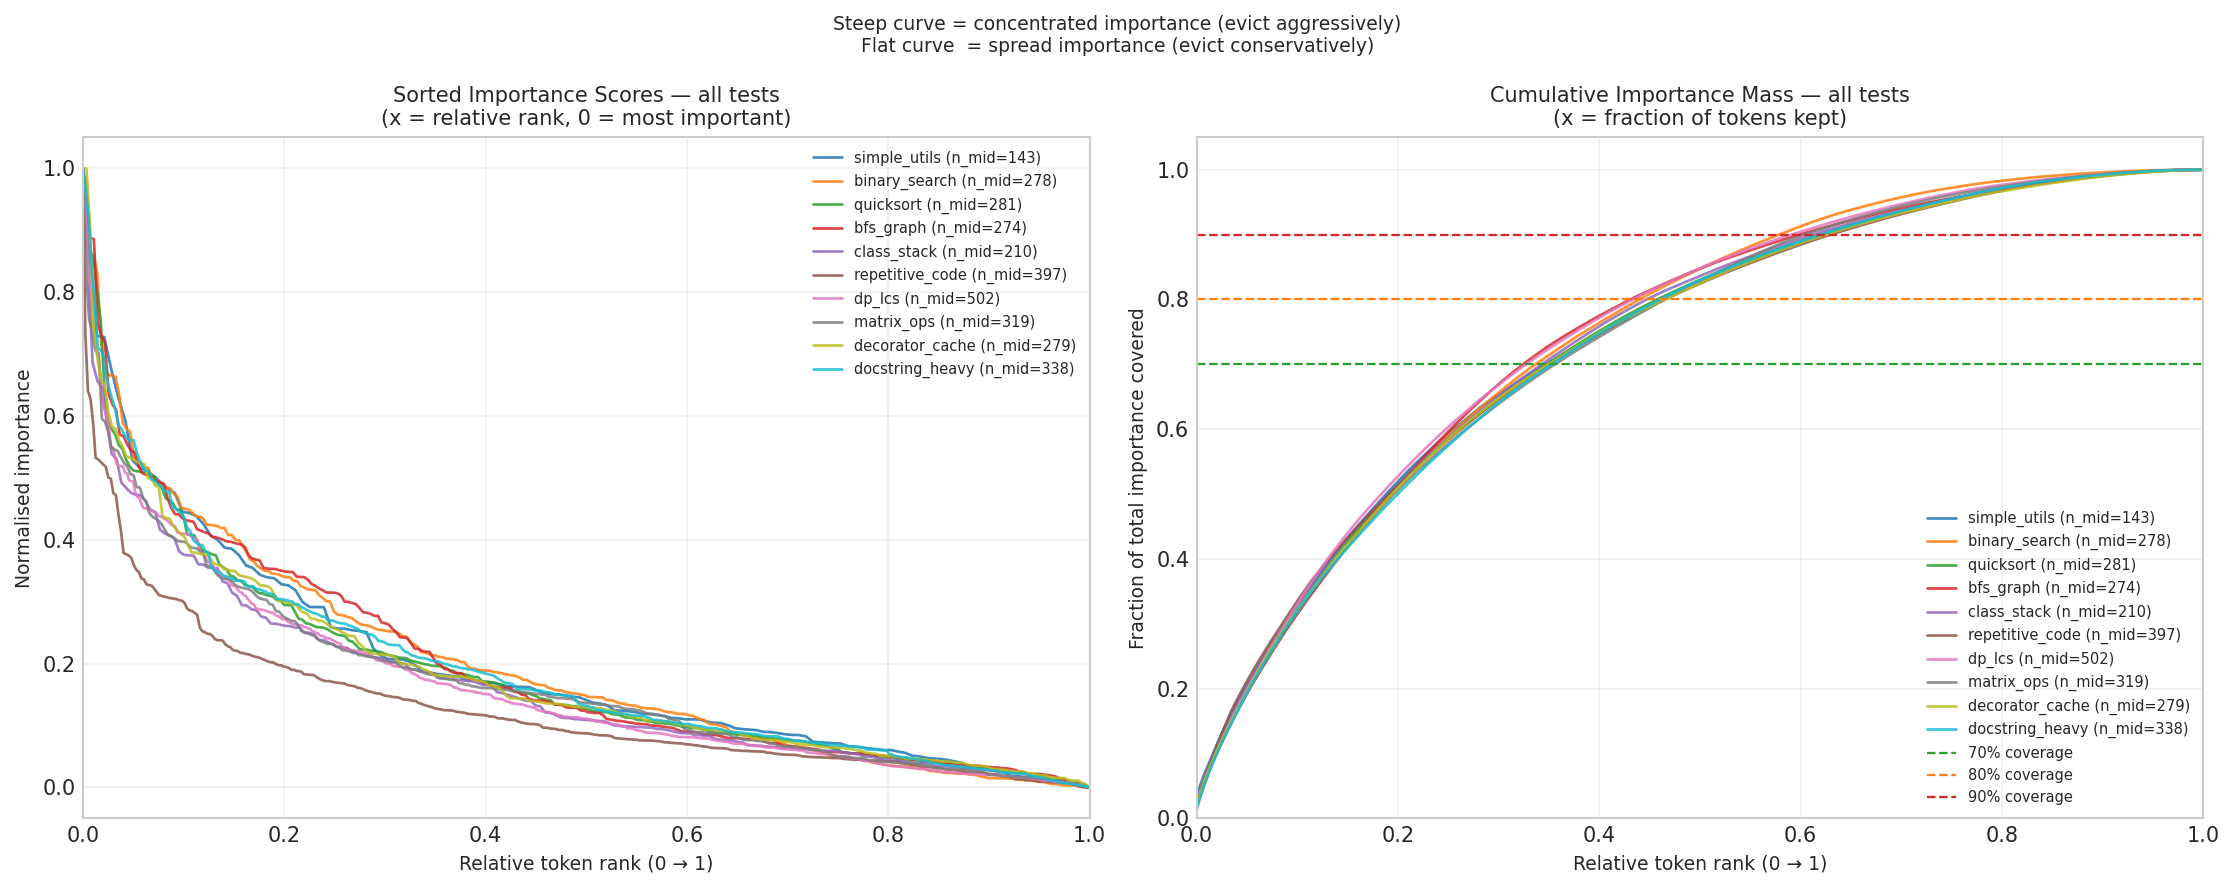
\includegraphics[width=\linewidth]{Figures/score_overlay.png}
  \caption{%
    Overlay of normalised importance-score curves (left) and cumulative-mass
    curves $C(k)$ (right) across ten code sequences of varying abstraction level.
    The $x$-axis is the relative token rank after sorting in descending importance
    order.  Dashed horizontal lines mark the 70\%, 80\%, and 90\% coverage thresholds.
    Steep score curves indicate concentrated importance and permit aggressive eviction;
    flat curves indicate near-uniform distributions and mandate conservative retention.%
  }
  \label{fig:score_overlay}
\end{figure*}



We observe that across all ten sequences, the sorted score curve falls steeply from a sharp peak
and flattens toward zero well before the full token budget is exhausted.
In every case, fewer than 30\% of mid-range tokens account for more than 80\% of
the total importance mass.  This confirms that the L-shaped long-tail decay
described in Section~3 is a robust structural property of MLA importance scores on
code corpora. And it is not an artefact of any particular program structure.


While all curves share the same qualitative shape, the degree of
concentration varies substantially.  Algorithmically dense sequences
(\texttt{quicksort}, \texttt{dp\_lcs}, \texttt{decorator\_cache}) exhibit steeper
decays and require only 15--25\% of tokens to reach 80\% cumulative mass.
By contrast, repetitive or comment-heavy sequences
(\texttt{repetitive\_code}, \texttt{docstring\_heavy}) produce shallower curves,
requiring 35--50\% retention for the same coverage level.
So a fixed compression ratio cannot simultaneously respect both extremes. A ratio
calibrated for concentrated sequences over-evicts the flat-distribution cases,
while a ratio calibrated for uniform sequences wastes memory on the concentrated
ones.  The variability in Figure~\ref{fig:score_overlay} therefore
directly motivates the knee-detection and coverage-floor mechanism of
Eq.~\eqref{eq:budget}.


For the flattest curves, the knee point
$k_\mathrm{knee}$ (Eq.~\eqref{eq:knee}) alone would settle near $k/n \approx 0.45$,
discarding a non-negligible fraction of uniformly-distributed importance mass.
The coverage floor $k_\mathrm{cov}$ (Eq.~\eqref{eq:cov}, $\tau=0.85$) acts as a
safety net, raising the effective budget to at most the 85\% mass threshold for
these sequences.  Conversely, for the steepest curves the coverage floor is
already satisfied at $k/n < 0.20$, so the knee criterion takes over and permits
aggressive eviction without triggering the floor.  This complementary interaction
validates the $\max(k_\mathrm{knee}, k_\mathrm{cov})$ formulation of the adaptive
budget. In the following experiment, $\tau$ is a parameter which can be chosen according
to different models or tasks. For example, \texttt{committee\_c85} means $\tau$ is 0.85 
and \texttt{committee\_c90} means $\tau$ is 0.9.







\bibliography{aaai2027} % Use aaai2027.bib (BibTeX expects filename without .bib)

% Check whether the conference requires a reproducibility checklist to be included in the paper.
% If so, you can uncomment the following line and ajust the path to include it.
% \input{ReproducibilityChecklist.tex}

\end{document}
